% Chapter 6

\chapter{Problems}
\label{Chapter6} 
By identifying  the requirements, we could then be able to highlight the related problems that we had to face in order to fulfill all of them. We will describe the related requirement as source of each faced problem.

\section{Mobile platform fragmentation}
Considering the requirement of a wide platform compatibility, we obviously need to face a really big problem in the mobile application world: the platform fragmentation.\\
Starting from the first smartphone release on 2007, the iPhone from Apple,  the sale of such devices keeps increasing each year. Between 2007 and 2008 sales proceeded upwards reaching the same sale rate of their computing parent, the PC. On 2009  the market signed an important inflection point, representing the beginning of an inexorable vertical rise. Although PCs were still the only ones to offer some types of functionality due to their longer replacement cycle, they were sold with a ratio of 1 : 2, compared to smartphones, over a 5 year period. This new market’ growth leads to an obvious seeking of various participants, some by choice and some by necessity, in order to extract value. Android has been the prime beneficiary, having been announced on 2007 and having gone on to account for well over half of smartphone sales worldwide. Apple, meanwhile, has maintained a steady ship, leveraging its skill in product design and user experience with a finely honed marketing machine, attracting a customer that rarely defects.\cite{ref5}
\begin{figure}[ht!]
	\centering
	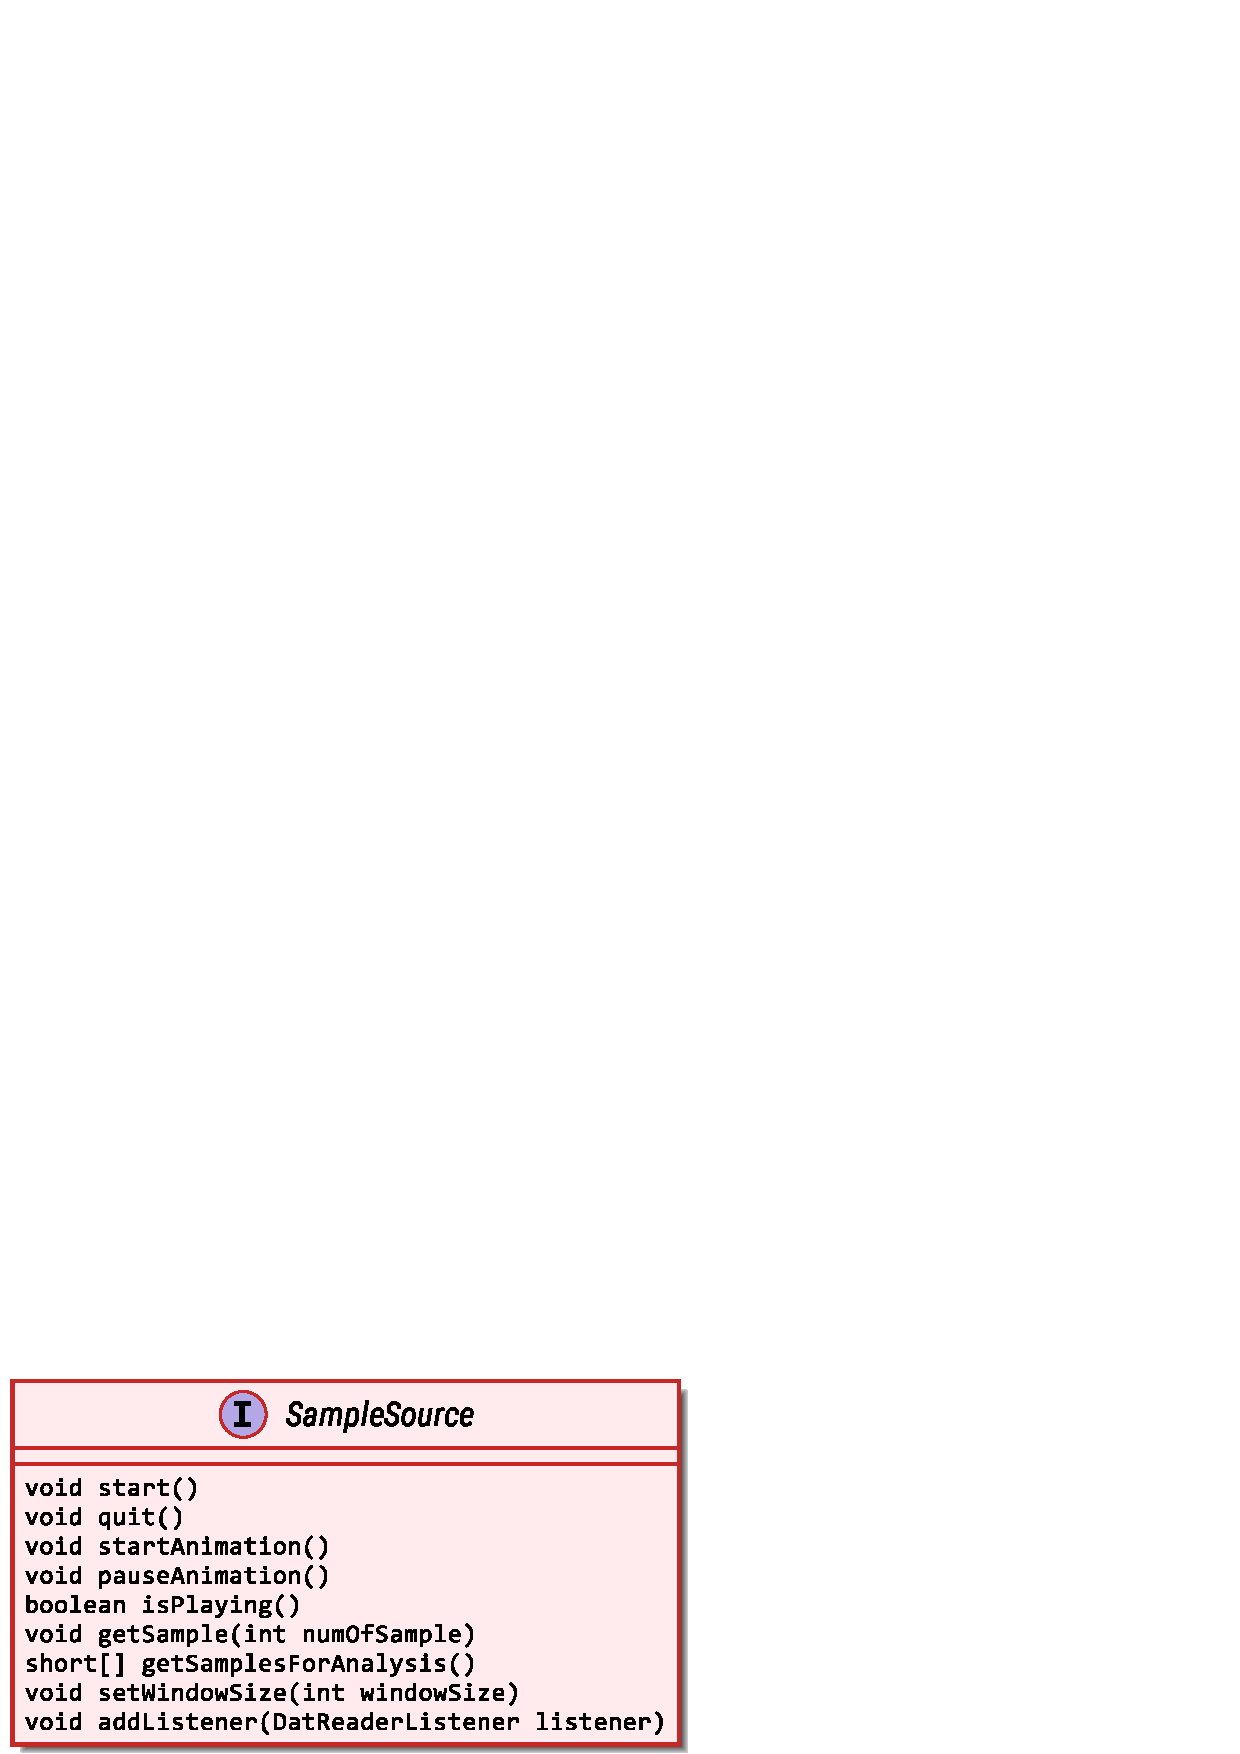
\includegraphics[width=120mm]{figures/ch6/1.png}
	\caption{Mobile platform share evolution (smartphone sales), 2009–13.}
	\label{fig6.1}
\end{figure}
Fast-forwarding to 2016, if we consider the global market share held by the leading smartphone operating systems, at first position we have Android with a share of  80.7\%, followed by iOS with a 17.7\%. Minor percentages are represented by Windows Phone (1.1\%), RIM (0.2\%) and others (0.2\%).\cite{ref6}

\section{Native vs Cross-Platform}
As mentioned earlier, one of the main challenges when moving to a mobile solution is the software development within a technology landscape that is highly fragmented and rapidly evolving. Mobile apps require a fair amount of customization to run on diverse platforms and a constant update due to the steady stream of new hardware, OS versions and browsers. Even a single platform (Android, Windows, Blackberry, and to a lesser extent Apple) has numerous flavors that require some degree of customization. There are also other factors such as the overlay software from different manufacturers that can affect behavior of an app on a particular device.\\
In response, the mobile industry has spawned a rapidly growing ecosystem of cross-platform and cross-device frameworks, source code analyzers, libraries of reusable components, and other tools designed to accelerate and simplify multi-platform development. New tools are constantly emerging, with new functionality, different capabilities,  strengths and weaknesses.\\
Developer’s preferences change and evolve, particularly as new tools and capabilities become available. However, the basic goals are the same: to code less and accomplish more, to reuse and recycle across multiple platforms as much as possible, and consider developing from scratch as the last resort. In addition, any tool or framework should be able to work with current and future evolving offers, and not to be locked because of a particular platform or technology.\cite{ref7}

\subsection{Native}
Native app development involves developing software specifically designed for a specific platform, hardware, processor and its set of instructions. Typical programming language are  Java, Object C,  Swift, C\# and many other.\\
Native apps’ major advantage over cross-platform apps is the ability to leverage device-specific hardware and software. This means that native apps can take advantage of the latest technology and API available on the mobile devices and it can well interface with other platform apps. Other advantages are a predictable increase on performance, streamlined support, native UI, native API and coherent library updates. However, the mobile platform’s fragmentation makes the task of keeping up with the pace of emerging technology onerous and costly, having to develop different software for each of the different platforms (Android, iOS, Windows Phone, Symbian).\\
Going further on a more technical analysis, native applications are represented by  executable binary files that will be installed into devices without the need for other abstraction layering to the operating system. They are able to call built in functionalities such as calendar, notifications, the dialer, email provider and others services and functionalities provided natively by the OS. Despite the fact that native applications development requires platform specific skill and expertise, this strategy delivers a higher quality user experience than other mobile application development methods (cross-platform or hybrid approach). Native apps are also best distributed through an app store.\cite{ref8}
\begin{figure}[ht!]
	\centering
	\includegraphics[width=100mm]{figures/ch6/2.png}
	\caption{Native app development process.}
	\label{fig6.2}
\end{figure}

\subsection{Cross-Platform}
Cross platform development produces one code base to maintain and write targeting multiple devices and platforms. It promises lower time of development and costs. The main categories of this group are web, hybrid, interpreted and generated apps. None of the previous is neither prevalent nor the best solution to the problem of developing cross-platform mobile applications.
\begin{figure}[ht!]
	\centering
	\includegraphics[width=120mm]{figures/ch6/3.png}
	\caption{Native vs Cross-Platform cost and time factors.\cite{ref9}}
	\label{fig6.3}
\end{figure}  
The main benefits of cross-platform development are:
\begin{itemize}
	\item Reduction of required skills to develop applications due to the use of common programming languages;
	\item Reduction of coding work, because the source code is written once and it is compiled for each supported OS;
	\item Reduction of development time and long term maintenance costs;
	\item Decrement of API knowledge, because with these tools is not needed to know the API’s of each OS, but only the API’s provided by the selected tool.\cite{ref10}
\end{itemize}

\section{Mobile hardware limitations}
As this project started from a previously developed desktop application, we needed to take into account all the limitation of mobile devices hardware. Despite the trend of mobile hardware is a constant increasing in computational power and memory availability, we cannot compare it with the one available nowadays in PC architectures, as the architectures on this two platforms are totally different: most of all pc are based on x86 architectures, whereas mobiles rely on ARM architectures. Furthermore, we could not commit the error of targeting only recent devices as they represent only a small percentage of all devices in the market, and it would have been in contrast to our main goal, which is a wide device compatibility.  We will discuss briefly about memory and computational differences in these type of architecture in the next paragraphs.

\subsection{Memory limitations}
The first point to consider is the device memory limitation. In the previous desktop application not so much effort was spent to reduce memory allocation: all the ECG record samples were allocated in memory both during acquisition and record opening. This approach could result convenient considering its low implementation effort, but it could be source of lots of problem when moving to a mobile device, where not only the physical memory are often small, but also the memory reserved to an application is limited (figure \ref{fig6.4}), both due to the coexistent apps running in the system and the power management of the mobile OSs. So we needed to find a good approach in order to manage these problems and not to face with memory leakages.
\begin{figure}[ht!]
	\centering
	\includegraphics[width=120mm]{figures/ch6/4.png}
	\caption{Memory reserved to an app in Android.}
	\label{fig6.4}
\end{figure}

\subsection{Performance limitations}
Talking about cpu computational power there is a huge gap between the two architectures.. Not considering the evident difference for what regarding the space availability for the CPU package, the main difference is that ARM architectures are focused on reducing the power consumption, a crucial characteristic in mobile devices. A technical report analyzed the execution time of a benchmark using a cross-platform version of WebKit showed that the tested ARM A9 architecture had a ratio of 5.8 (normalized time) compared to the tested x86 architecture.\cite{ref11}

\section{ECG baseline wander}
For a right interpretation and identification of physiological and pathological phenomena, a low error is required in the ECG signal. But often ECG recordings are distorted by two main artifacts:
\begin{itemize}
	\item high-frequency noise caused by electromyogram induced noise, power line interferences, or mechanical forces acting on the electrodes;
	\item baseline wander (BW) that may be due to respiration or the motion of the patients or an instrument fault (Figure 6.5).
\end{itemize}
These artifacts strongly limit the utility, readability and interpretation of a recorded ECGs. In ECG enhancement, the goal is to separate the valid ECG from the undesired artifacts so that we can extract a signal that allows an easy visual interpretation.\cite{ref12}
The first class of artifact is mostly solved within the acquisition device at hardware low-level though filters and a proper settings. In this project we will deal with the second class of artifact which can be managed at software level.
\begin{figure}[ht!]
	\centering
	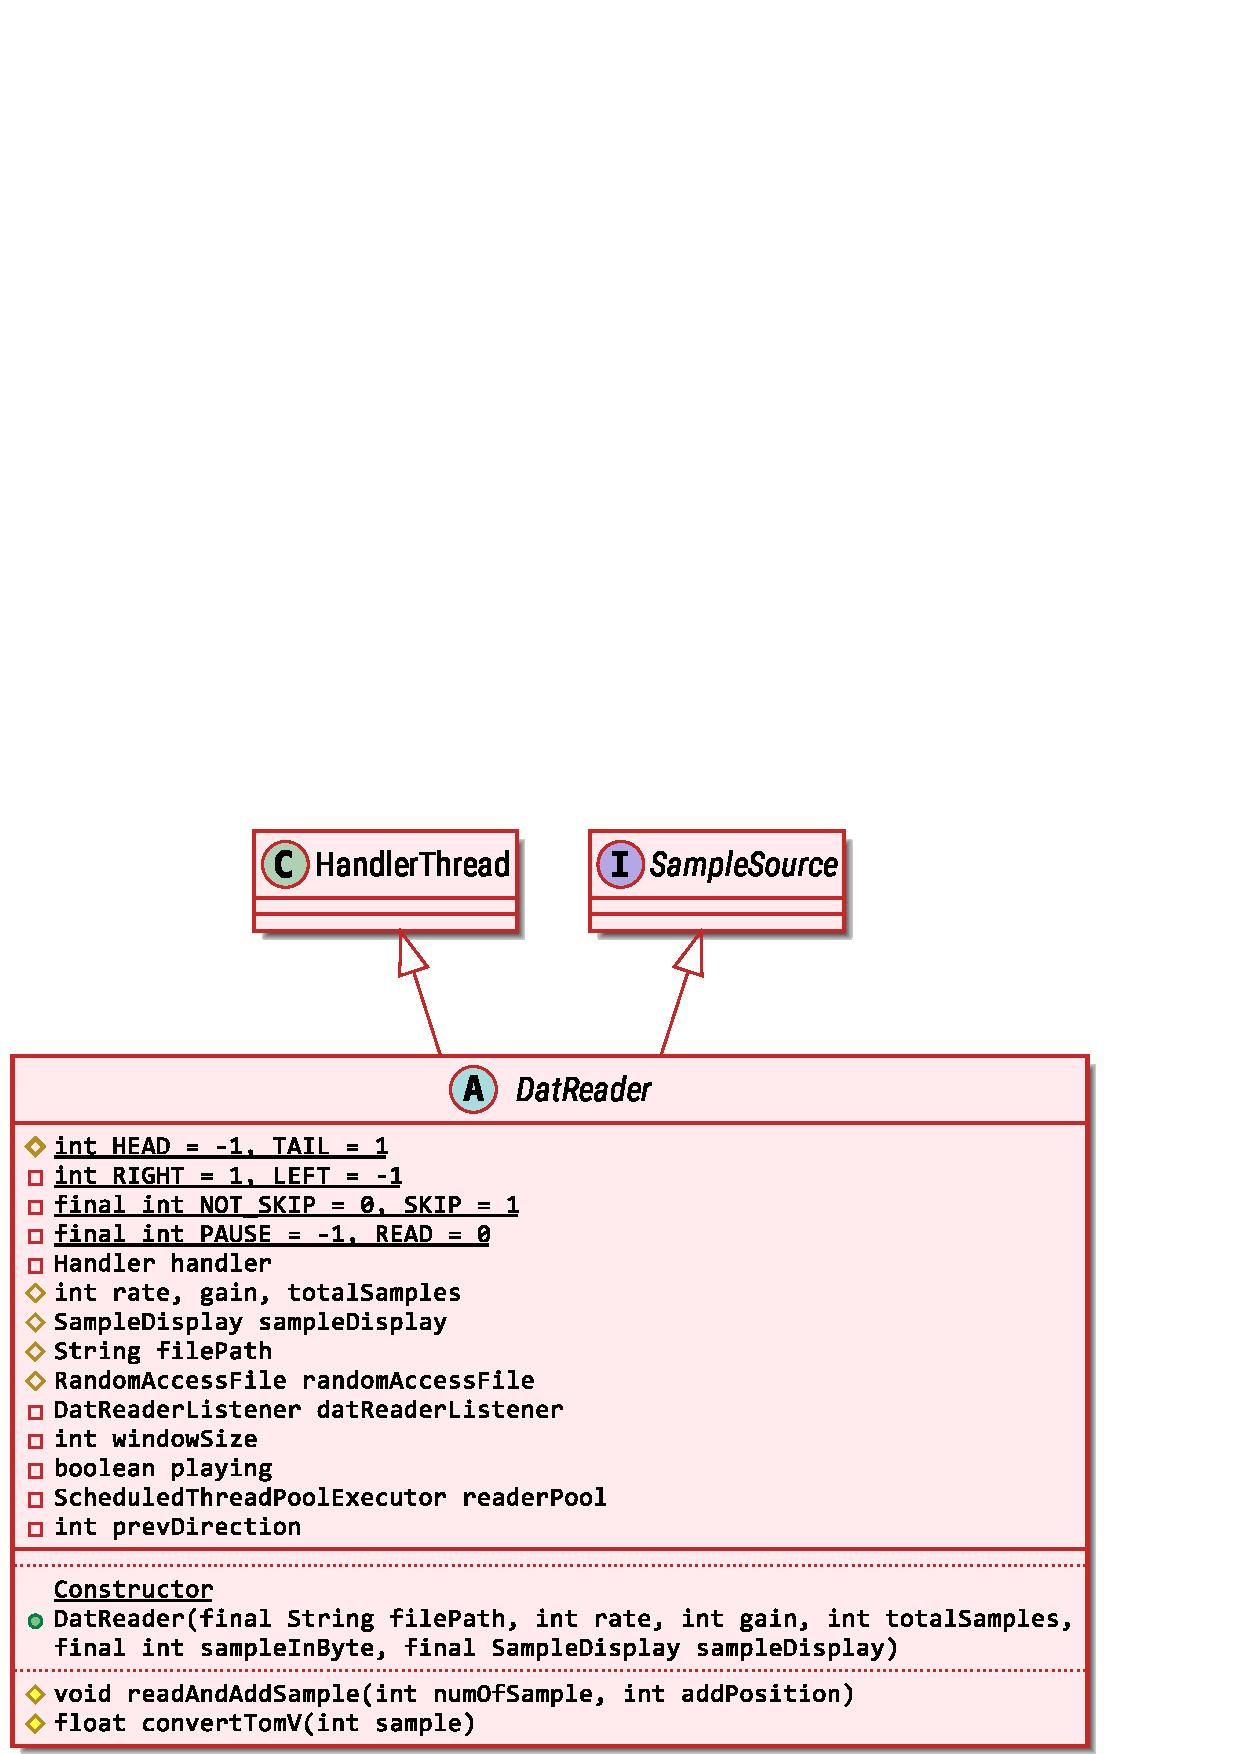
\includegraphics[width=110mm]{figures/ch6/5.png}
	\caption{The baseline wander artifact in the ECG signal.}
	\label{fig6.5}
\end{figure}

\subsection{State of Art}
Two methods, in recent years have often been applied to remove BW:
\begin{itemize}
	\item Polynomial fitting: in order to assess the baseline, it uses a polynomial interpolation. The baseline is fit from some fiducial points that are determined from P-R intervals, whereas these fiducial points are difficult to accurately locate before noise is removed from the ECG signal. As result this approach is ineffective if the ECG signal is contaminated by noise.\cite{ref13}
	\item High-pass filtering: to implement this type of filtering, usually a moving average filter\cite{ref14} and wavelet translation\cite{ref15}. This approach however would unavoidably introduce distortions in various parts of the ECG signal, especially in the ST segment due to the spectra of the ST segment that overlaps the spectra of BW.
\end{itemize}

\subsubsection{Simple Moving Average Filter}
This type of filtering is defined as
\begin{equation}
y(n)=\frac{1}{2N+1}\sum_{i=-N}^{N}x(n+i)
\end{equation}
where $x(n)$ and $y(n)$ are input signal and output signal of the moving average respectively, and $N$ specifies the observation window length equal to $2N+1$. So the baseline can be estimated as
\begin{equation}
z(n)=x(n)-y(n)
\end{equation}
where $z(n)$ is the output signal of the high-pass filter.

\subsubsection{Distortion using Simple Moving Average Filtering}
Obviously the baseline values estimated from the P-R segment (between 0.3 s and 0.6 s) are very close to real baseline values, while the baseline values estimated from segments including QRS complex and T wave are far away from the real baseline. Therefore, if an observation window covers some sample points with extreme amplitudes, an ECG signal would be distorted.

\subsubsection{CPU intensive operation}
Many methods are known in the literature that perform better and reduce the error in the ECG signal due to the filtering, like wavelet package translation filter\cite{ref16}, or the statistical weighted moving average filter\cite{ref17}. Defined the normalized root mean square error ($NRMSE$) and maximum error ($ME$) as
\begin{equation}
NRMSE=\sqrt{\frac{\sum_{i=1}^{L}(ecg_{in}(i)-ecg_{out}(i))^2}{\sum_{i=1}^{L}ecg_{in}(i)}}\end{equation}
\begin{equation}
ME=\max_{i=1,2,\dots,L}|ecg_{in}(i)-ecg_{out}(i)|
\end{equation}
The figure \ref{fig6.6} shows a comparison between the methods.
\begin{figure}[ht!]
	\centering
	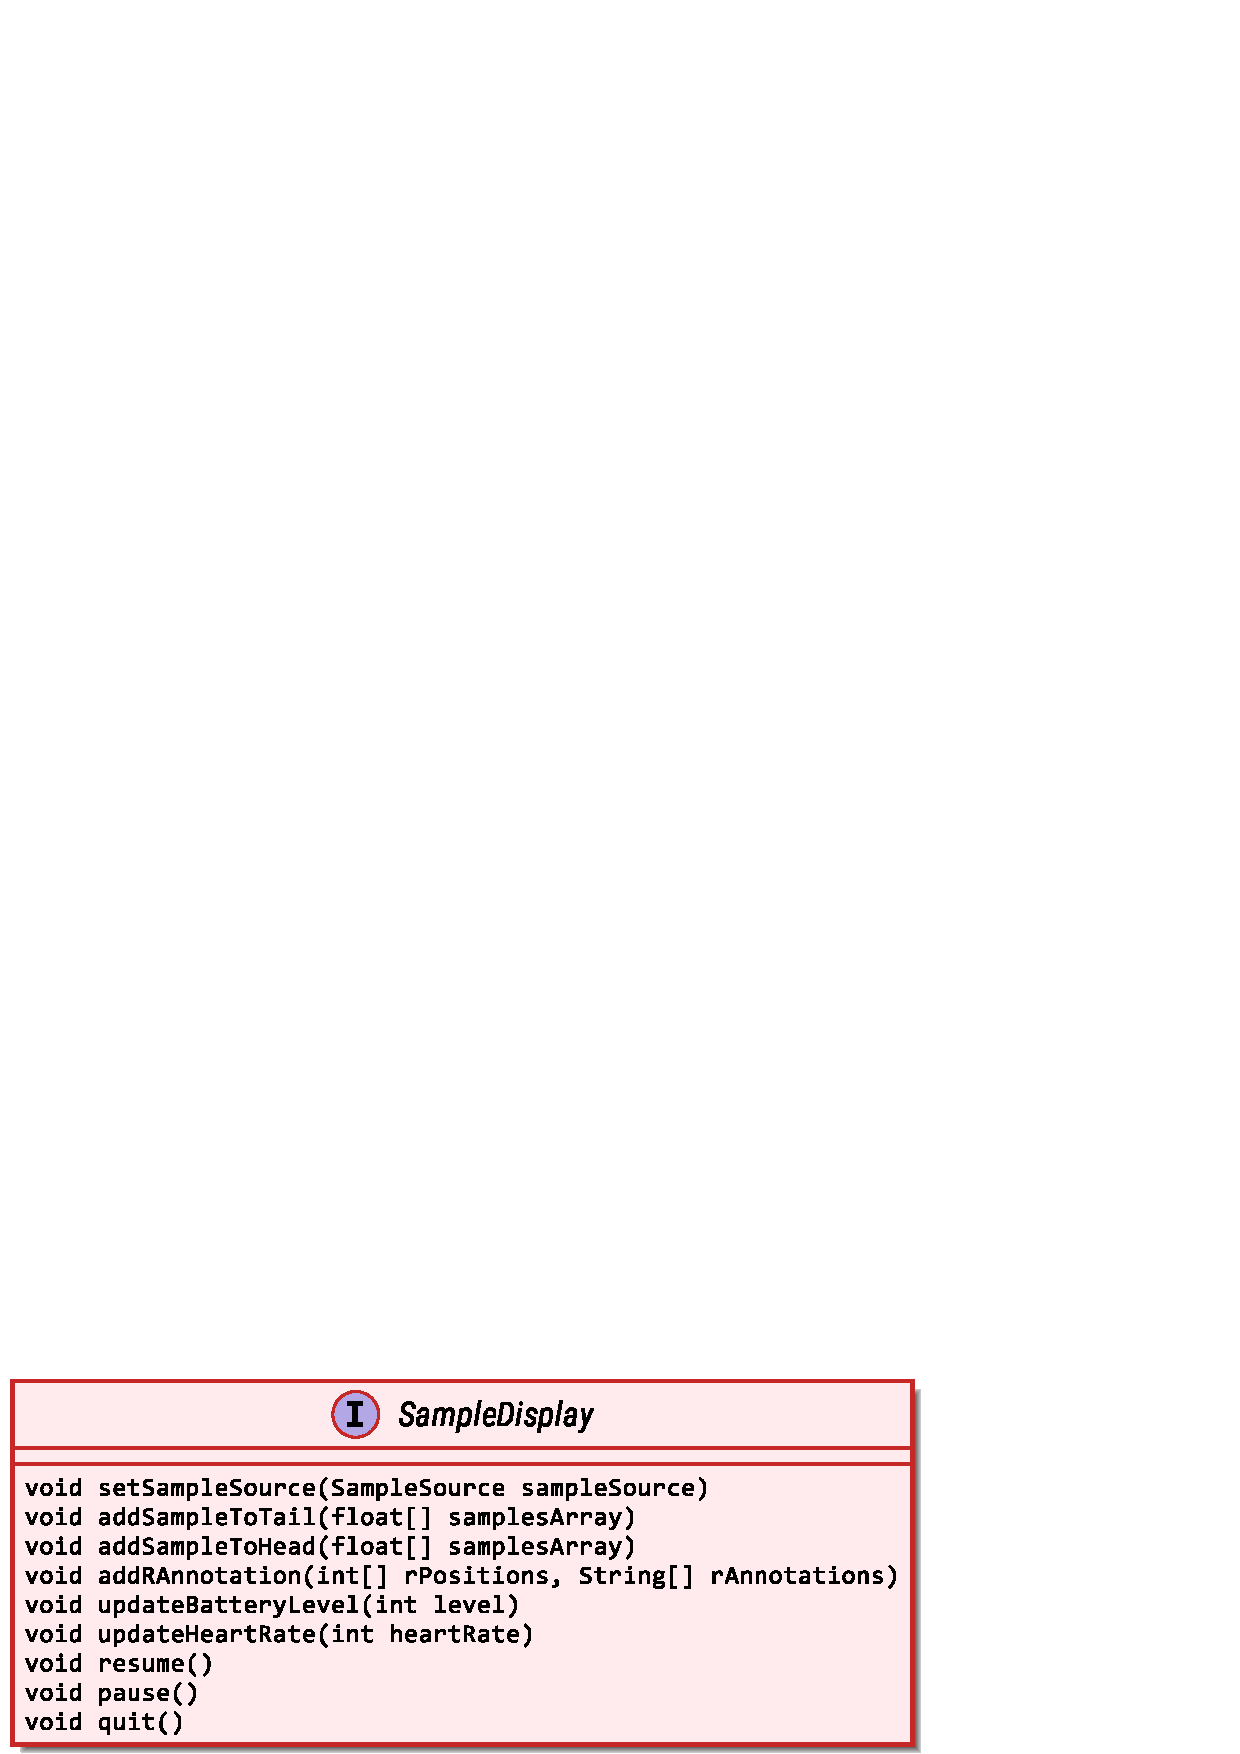
\includegraphics[width=110mm]{figures/ch6/6.png}
	\caption{Relation between distortion and moving window length for wavelet package translation (WPT), traditionally used MA, and our proposed high-pass filter based on a statistical weighted moving average (SMA).\\
		(a) Maximum error (ME) vs. moving window length;\\
		(b) Normalized root mean square error (NRMSE) vs. moving window length. M is the number of sub-bounds. SMA is the same as MA when M=1.}
	\label{fig6.6}
\end{figure}
Of course the computational complexity these advanced methods is really high. Considering that this type of filtering is supposed to be used during a real-time acquisition in our project, they are obviously prohibitive.

\section{Signal visualization}
The problem of an efficient ECG signal visualization shows up when the application has to plot samples of an acquisition device with a rate of 500Hz. Because of this the app has to be able to draw $500-1$ lines (connecting two samples) for each mapped second in the ECG paper grid. Taking into account the standard size of a second in the standard ECG paper of 5mm, and the fact that the visualization size has to respect this measure, if we consider a device screen of 4.6 inch in portrait, we have around 11 seconds of samples to visualize. Hence we have $(500 - 1) * 11 = 5489$ lines to plot. If we are supposed to plot ideally all the ECG derivation (12), the number of total lines become $5489 * 12 = 65868$. Now, this is the number of lines  we need to plot in order to cover the total visible window screen space. If we want to have a good display smoothness we must guarantee at least 30FPS (frame rate per seconds), ideally 60 frame/s (FPS). Assuming a minimum of 30 FPS we have a total of $65868 * 30 = 1976040.$\\
These numbers gives us an idea of the computational effort that is spent only only to plot the samples.